% PAKETE UND DOKUMENTKONFIGURATION
\documentclass[11pt, a4paper]{article}

% Encoding für Umlaute
\usepackage[utf8]{inputenc}
\usepackage[T1]{fontenc}

% Silbentrennung
\usepackage[ngerman]{babel}

% erweiterte Matheumgebungen und Formelnummer mit Sectionnummer
\usepackage{amsmath}
\numberwithin{equation}{section}

% Braket Notation
\usepackage{braket}
\usepackage{isotope}
\usepackage[version=4]{mhchem}
\usepackage{tensor}
\usepackage{slashed}

% zusätzliche mathematische Schriftarten
\usepackage{amsfonts}

% verschiedene mathematische Symbole
\usepackage{amssymb}

% Einheiten setzen z.B. \SI{10}{\kilo\gram\meter\per\second\squared}
% Fehler: \SI{10 +- 0,2e-4}{\metre}
\usepackage{siunitx}
\sisetup{
  output-decimal-marker={,},
  separate-uncertainty
}

% Einheitendefinitionen
\DeclareSIUnit{\skt}{Skt.}
\DeclareSIUnit{\gauss}{G}
\DeclareSIUnit{\division}{div.}
\DeclareSIUnit{\Kanal}{Kanal}

% Operatordefinitionen
\DeclareMathOperator{\erf}{erf}

% Randbreiten
\usepackage[left=3.5cm,right=3.5cm,top=3cm,bottom=3cm,twoside]{geometry}

% Bilder einfügen
\usepackage{graphicx}
\usepackage[percent]{overpic}

% Textfarbe
\usepackage{color}

% Verweise innerhalb des Dokuments
\usepackage{hyperref}
\hypersetup{
	colorlinks = true,
	allcolors = {black}
}

% bessere Tabellenlayouts
\usepackage{booktabs}
\usepackage{multirow}
\usepackage{multicol}

% Seitenlayout (Kopfzeile)
\usepackage{fancyhdr}

% Float Barriers
\usepackage{placeins}

% Pakete für gedrehte Subfigures
\usepackage{caption}
\usepackage{subcaption}
\usepackage{rotating}

% Paket für textumflossene Abbildungen und Tabellen
\usepackage{wrapfig}

\usepackage{float}

% Caption-Setup
\captionsetup{font={small}}
\renewcommand{\thefigure}{\thesection.\arabic{figure}}
\renewcommand{\thesubfigure}{\alph{subfigure}}
\renewcommand{\thetable}{\thesection.\arabic{table}}
\renewcommand{\thesubtable}{\alph{subtable}}

% Manuelle Silbentrennung
\hyphenation{Sekundär-elek-tronen-verviel-facher}

% Tiefe des Inhaltsverzeichnisses (Level: 1 sections, 2 subsections,
% 3 subsubsections)
\setcounter{tocdepth}{3}

% FANCYHDR SETUP
\pagestyle{fancy}
\fancyhead[EL,OR]{\thepage}
\fancyhead[ER]{\leftmark}
\fancyhead[OL]{\rightmark}
\setlength{\headheight}{13.6pt}

\renewcommand{\sectionmark}[1]{
\markboth{\thesection{} #1}{\thesection{} #1}
}
\renewcommand{\subsectionmark}[1]{
\markright{\thesubsection{} #1}
}

\newcommand{\korr}[1]{{\color{red}(#1)}}

% DOKUMENTINFORMATIONEN
\title{A248 \\ Magneto-optische Falle}

\author{Christopher Deutsch\footnote{christopher.deutsch@uni-bonn.de} \and Christian Bespin\footnote{christian.bespin@uni-bonn.de}}

\date{\today}

\begin{document}

\begin{titlepage}

\maketitle

% DURCHFÜHRUNGSDATUM UND TUTOR
\begin{center}
\begin{tabular}{l r}
Durchführung: & 4./5. April 2016 \\
Gruppe: & P8 \\
Tutor: & Daniel Babik
\end{tabular}
\end{center}

% ZUSAMMENFASSUNG
\begin{abstract}
\noindent
\end{abstract}

\end{titlepage}

% INHALTSVERZEICHNIS
\tableofcontents
% Neue Seite nach TOC
\newpage

% INHALT VERSUCHSPROTOKOLL
\section{Einführung}

\section{Theorie}

\section{Aufbau der MOT}
A -- I (Durchführung \& Messungen)



\section{Charakterisierung der MOT}
\label{sec:charakterisierung_mot}
Nachdem die MOT aufgebaut und auf möglichst hohe Fluoreszenz optimiert wurde, kann im Folgenden die Charakterisierung einiger Eigenschaften der Falle durchgeführt werden.

\subsection{Atomzahl in der MOT}
Im Folgenden soll die Anzahl der gefangenen Atome in der MOT bestimmt werden.
Dazu muss zunächst der Fluoreszenzleistung der gefangenen Atome und der Strahlradius des Lasers bestimmt werden.


\subsubsection{Fluoreszenz der MOT}
Zur Bestimmung der Fluoreszenz der MOT wird die leuchtende Atomwolke mithilfe einer Linse auf ein Leistungsmessgerät abgebildet.
Dabei gilt es zu beachten, dass die so gemessene Leistung auch die Fluoreszenz von ungefangenen Atomen beinhaltet.
Daher wird nach jeder Messung das Magnetfeld der Falle deaktiviert um eine Hintergrundmessung durchzuführen und der so gemessene Hintergrund kann vom Fluoreszenzsignal abgezogen werden.
Somit wird die Fluoreszenzleistung, die die Atomwolke in dem von der Linse aufgespannten Raumwinkel emittiert, zu
\begin{align*}
	P_\mathrm{Linse} = \SI{114 +- 5}{nW}
\end{align*}
bestimmt.
Um die Fluoreszenzleistung zu erhalten, die im gesamten Raumwinkel von~$4\pi$ emittiert wird, kann
\begin{align*}
	P_\mathrm{tot} = P_\mathrm{Linse} \cdot \frac{A_\mathrm{tot}}{A_\mathrm{Linse}}
\end{align*}
genutzt werden.
Dabei beschreibt $A_\mathrm{Linse}$ die Fläche der Linse und $A_\mathrm{tot}$ die Oberfläche der Kugel mit einem Radius $R$, der dem Abstand der MOT zur Linse entspricht.
Somit erhält man
\begin{align*}
	P_\mathrm{tot} = P_\mathrm{Linse} \cdot \frac{4 \pi R^2}{\frac{1}{4} \pi d_\mathrm{Linse}^2} = P_\mathrm{Linse} \cdot \frac{16 R^2}{d_\mathrm{Linse}^2}
\end{align*}
und mit den gemessenen Werten für den Linsendurchmesser
\begin{align*}
	d_\mathrm{Linse} = \SI{2.5 +- 0.1}{cm} \, \text{,}
\end{align*}
sowie dem Abstand~$R$ zwischen MOT und Linse
\begin{align*}
	R = \SI{10.3 +- 0.2}{cm}
\end{align*}
kann die gesamte Leistung berechnet werden.
Diese ergibt sich zu
\begin{align*}
	P_\mathrm{tot} = \SI{30.9 +- 3.1}{\micro\watt} \, \text{,}
\end{align*}
wobei der Fehler durch \textsc{Gauß}sche Fehlerfortpflanzung gemäß
\begin{align*}
	\Delta P_\mathrm{tot} = \frac{16}{d_\mathrm{Linse}^3} \sqrt{4 R^2 P_\mathrm{Linse}^2 d_\mathrm{Linse}^2 \Delta R^2 + R^4 \left( d_\mathrm{Linse}^2 \Delta P_\mathrm{Linse}^2 + 4 P_\mathrm{Linse}^2 \Delta d_\mathrm{Linse}^2 \right)}
\end{align*}
berechnet wurde.


\subsubsection{Strahlradius des Lasers}
Anschließend muss eine Bestimmung des Strahlradius durchgeführt werden.
Dazu wird das Leistungsmessgerät in den Strahlengang gestellt und der Laser wird seitlich durch eine Messerklinge blockiert.
Durch eine Messung der Leistung des teilweise blockierten Laserstrahls in Abhängigkeit der Position der Klinge kann der Strahlradius bestimmt werden.
Dazu wird angenommen, dass der Laserstrahl durch einen \textsc{Gauß}-Strahl beschrieben werden kann, weshalb die Intensität des Strahls in der transversalen Ebene durch
\begin{align*}
	I(x, y) = \frac{2 P_0}{\pi w^2} \exp\left( - \frac{x^2 + y^2}{w^2} \right)
\end{align*}
mit der Gesamtleistung des Strahls~$P_0$ und dem Strahlradius~$w$ gegeben ist.
Durch Integration kann nun die Leistung des teilweise blockierten Strahls bestimmt werden
\begin{align*}
	P(x) &= \int_{x}^{\infty} \mathrm{d}x^\prime \int_{-\infty}^{\infty} \mathrm{d}y^\prime \, I(x^\prime, y^\prime) \\
	     &= \frac{P_0}{2} \left[ 1 - \erf\left( \frac{\sqrt{2} x}{w}\right) \right] \, \text{,}
\end{align*}
wobei $x$ den von der Klinge blockierten Teil des Strahls beschreibt.


\begin{figure}[h]
	\centering
	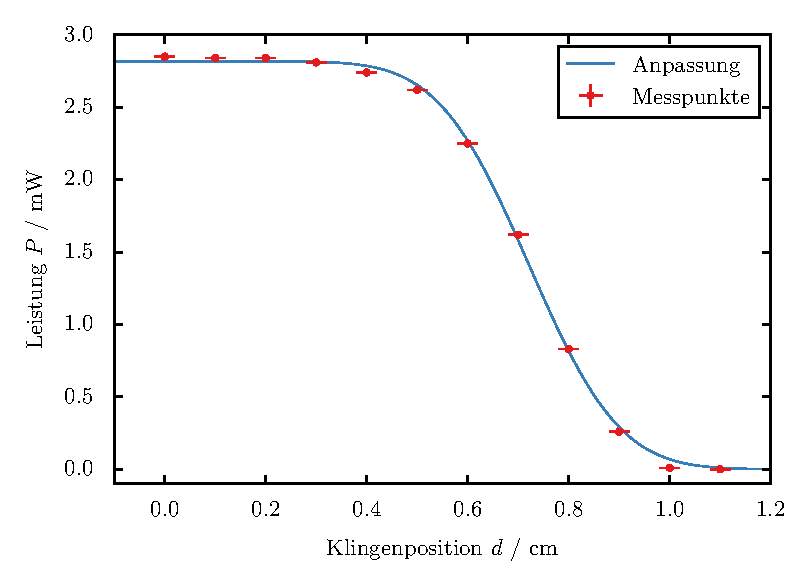
\includegraphics{./figures/beam_radius_fit.pdf}
	\caption{Anpassung des Strahlradius}
\end{figure}



\subsection{Größe der MOT}


\subsection{Einfluss der $\lambda / 4$-Platten}


\subsection{Einfluss des Magnetfeldes}


\subsection{Verhalten des Ladevorgangs}


\subsection{Verstimmung der Laserfrequenzen}






\section{Fazit}


\FloatBarrier
% BIBLIOGRAPHIE
\vspace{\fill}
% Maximale Anzahl der Einträge in Klammer
% Zitieren mit \cite{lamport94}
\begin{thebibliography}{19}
\bibitem{anleitung}
	\emph{Advanced Laboratory Course (physics601): Description of Experiments}, BONN-AT-2016-01MP, Universität Bonn, Januar 2016
\end{thebibliography}

% APPENDIX
\begin{appendix}
\newpage
\section{Anhang}
\end{appendix}

\end{document}
